\section{Dato per scontato\\ anche se mai imparato}
Questa sezione è dedicata a chi ha bisogno di un ripasso di elementi non spiegati nel corso ma comunque necessari per gli argomenti del corso.
\subsection{Disequazioni}
 Queste sono le formule per dire quando $y=ax^2+bx+c$ con $a>0$ è positivo. Le formule per $a<0$ si ricavano moltiplicando per $-1$ le sequenti formule:
 
 \begin{gather*}
 \Delta>0 \quad \f (x)\quad x<x'\quad \cup x>x''\\
 \Delta=0 \quad \forall x \in \text{Dominio}\\
 \Delta>0 \quad \forall x \in \text{Dominio}\\
 \end{gather*}

\begin{wrapfloat}{figure}{r}{0pt}
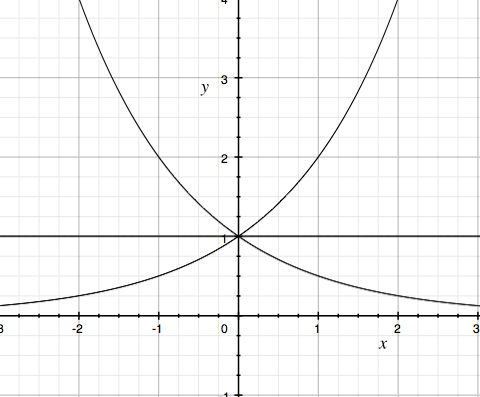
\includegraphics[width=0.5\columnwidth]{Esponenziale}
\caption{Funzioni esponenziali con $a>1$, $a=1$ e $a<1$}
\end{wrapfloat}

\subsection{Esponenziale e logaritmi}

Si può vedere dalla figura che $a^x$ è decrescente se $0<a<1$ ed è crescente se $a>1$. Se $a=1$ il grafico è quello della retta $y=1$.
La funzione esponenziale \f$:x\to a^x$ è monotona quindi invertibile. Infatti la sua inversa è la funzione logaritmo in base a di x e si indica con \f$^-1 :x \to \lg_a x$.
Il logaritmo in base a di x è l'esponente di a che serve per ottenere x.\\
 \newline
 \paragraph{NB:}
  \begin{gather}
   {\lg}_a 1=0\\
   {\lg}_a a=1\\
   {\lg}_a (xy)= {\lg}_a x + {\lg}_a y\\
   {\lg}_a (\frac{x}{y}={\lg}_a x - {\lg}_a y\\
   {\lg}_b x=\frac{{\lg}_a x}{{\lg}_a b}
  \end{gather}

 \subsection{Trigonometria}
\begin{wrapfloat}{figure}{r}{0pt}
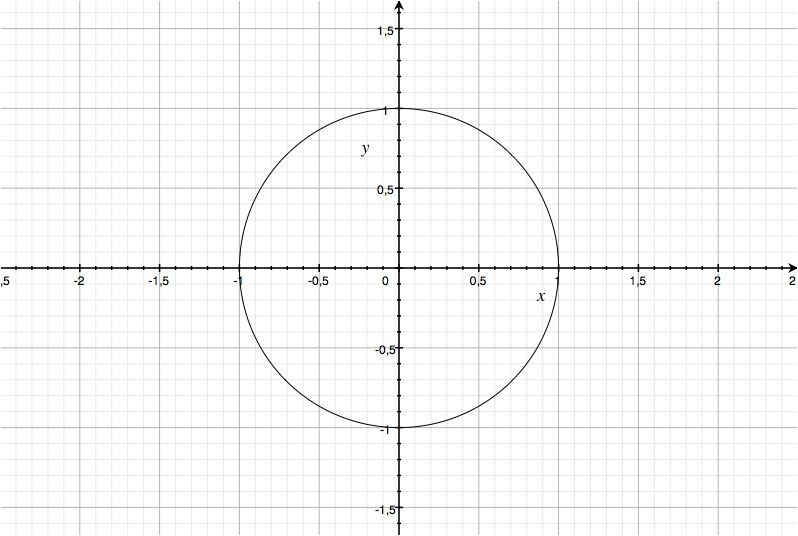
\includegraphics[width=0.5\columnwidth]{Trigonometria}
\caption{Circolo goniometrico}
\end{wrapfloat}
La trigonometria si basa tutto sul circolo goniometrico, circonferenza di raggio unitario (fig 1.2) su cui si disegnano gli angoli con cui si lavora.
La trigonometria usa come misura degli angoli i \textit{radianti} ovvero la misura dell'angolo che sottende un arco di circonferenza uguale al raggio. Per convertire dai gradi basta ricorrere alla seguente proporzione:
\[
\text{gradi}:360=\text{radianti}:2\pi
\]

La tabella mostra~gli angoli notevoli in gradi e radianti.\\

\[\begin{array}{cc}
\toprule
Gradi   & Radianti \\
\midrule
30 & \frac{\pi}{6} \\
60 & \frac{\pi}{3} \\
45 & \frac{\pi}{4} \\
90 & \frac{\pi}{2} \\
180 & \pi \\
270 & \frac{3}{2}\pi \\
360 & 2\pi \\
\bottomrule
\end{array}\]
 

 \paragraph{Seno e Coseno}
 Dato l'angolo orientato $\alpha=\widehat {aop}$ si definiscono $\sin$ e $\cos$ di $\alpha$ rispettivamente come l'ordinata y e l'ascissa x del punto~$\mathbb{P}$:
 \[
 \sin \alpha =yp
 \text{ e }
 \cos \alpha =xp
 \]
 
\paragraph{NB:}
 \begin{gather}
    \sin(\frac{\pi}{2})-\alpha=\cos\alpha\\
    \cos(\frac{\pi}{2}-\alpha)=\sin\alpha\\
    \sin(\frac{\pi}{2}+\alpha)=\cos\alpha\\
    \cos(\frac{\pi}{2}+\alpha)=-\sin\alpha\\
    \sin(\pi-\alpha)=\sin\alpha\\
    \cos(\pi-\alpha)=-\cos\alpha
 \end{gather}
 
 Altre formule utili della trigonometria:
 
 \begin{form}[Ugualianza fondamentale]
 \[
 \sin^2(\alpha)+\cos^2(\alpha)=1
 \]
 \end{form}
 
 \begin{form}[Addizione-sottrazione seno]
 \[
 sen(x\pm y)=\sin x \cos y\pm\cos x \sin y
 \]
 \end{form}
 
 \begin{form}[Addizione-sottazione coseno]
 \[
 \cos(x\pm y)=\cos x\cos y\pm\sin x \sin y
 \]
 \end{form}
 
 \begin{form}[Duplicazione seno]
	\[
	\sin 2x=2\sin x\cos x
	\]
 \end{form}
 
 \begin{form}[Duplicazione coseno] 
\[
\cos^2 x-\sin^2 x
\]
 \end{form}
 
 \begin{form}[Prostaferesi seno]
 \[
 \sin x \pm \sin y=2\sin(\frac{x\pm y}{2}) \cos(\frac{x \pm y}{2})
 \]
 \end{form}

 \begin{form}[Prostaferesi coseno]
 \[
 \cos x +\cos y=+2\cos(\frac{x+y}{2})\cos(\frac{x-y}{2})
 \qquad
 \cos x -\cos y=-2\sin(\frac{x+y}{2})\sin(\frac{x-y}{2})
 \]
 \end{form}
 
 \paragraph{Tangente}
 La \textit{tangente} non è altro che $\frac{\sin x}{\cos x}= \tan x$. Le formule riportate qui sopra permettono di ricavare le formule equivalenti per la funzione tangente.
 
 \paragraph{Altre funzioni trigonometriche}
 Sono \textit{secante, cosecante} e \textit{cotangente}.  Esse sono delle funzioni derivate da quelle viste fin ora:\\
\begin{gather}
 \sec x=\frac{1}{\cos x}\\
 \cos x=\frac{1}{\sin x}\\
 \cot x=\frac{1}{\tan x}\\
\end{gather} 

